\documentclass[10pt,twocolumn]{article}

\usepackage[margin=2cm]{geometry}
\usepackage{lmodern} 
\usepackage[T1]{fontenc}
\usepackage{graphicx}
\usepackage{booktabs}
\usepackage{hyperref}

\usepackage{amsmath}
\usepackage{amssymb}
\usepackage{mathtools}
\usepackage{amsthm}
\newcommand{\Cref}[1]{Figure~\ref{#1}}

\title{Geometry of Superposition in a Toy Model and SAE Recovery \\[6pt]
       \normalsize Homework 7 --- Research in LLMs, HSE x Central University}
\author{Ivan A. Novosad \\ \texttt{inovosad@hse.ru}}
\date{}

\begin{document}
\maketitle

\begin{abstract}
I study how a toy ReLU autoencoder ($F$ features compressed into $d$ dimensions)
learns superposition, and how well a vanilla Sparse Autoencoder recovers the
ground-truth features. Three findings stand out. First, at $d{=}2$ the model
discovers clean polytope structures (digons, triangles, pentagons) that transition
discretely as $F$ increases. Second, SAE reconstruction quality (EV $> 0.97$ for most configurations,
dropping only under aggressive sparsity) is a poor proxy for feature recovery: high EV
coexists with weighted MMCS as low as 0.80. Third, rare features are
systematically lost by the SAE, with a sharp frequency threshold separating
recovered from unrecovered features.
\end{abstract}

% ===================================================================
\section{Setup}
\label{sec:setup}

The toy model and SAE follow the assignment specification exactly. One
implementation note: the EV formula includes a square root,
$\text{EV} = 1 - \sqrt{\text{Var}(h - \hat{h}) / \text{Var}(h)}$,
which is stricter than the standard $R^2$.

\paragraph{Weighted MMCS.}
Vanilla MMCS is misleading when some features have near-zero norm. If the model
assigns $\|W_i\| \approx 0$ to a rare feature (effectively not representing it),
the cosine similarity with any dictionary element is undefined or arbitrary ---
yet it still contributes equally to the average. I introduce weighted MMCS:
each feature's max-cosine is weighted by $\|W_i\| / \max_j \|W_j\|$.
Features the model does not represent contribute proportionally less.
In practice, weighted MMCS and vanilla MMCS agree when $F/d$ is small
(all features represented), but diverge at high superposition where many
features have negligible norm.

\paragraph{Experimental details.}
Default configuration: $F{=}50$, $d{=}5$, $\alpha{=}1.0$, 10k toy model
training steps, 20k SAE steps, batch size 1024, Adam optimizer, $F_{\text{SAE}}{=}100$,
$\ell_0{=}0.1$, 10\% L1 warmup. All sweeps use 3 seeds (42, 43, 44) and
report mean $\pm$ std.

% ===================================================================
\section{Part 1: Geometry of Feature Embeddings}
\label{sec:geometry}

\subsection{Polytope Structures at $d{=}2$}
\label{sec:polytope}

\textbf{Hypothesis:} When $d{=}2$, the model should discover discrete geometric
arrangements to pack $F > 2$ features into a 2D space, forming structures
analogous to solutions of the Thomson problem (placing repulsive charges on a
circle).

I trained models with $F \in \{4, 5, 6, 8, 10\}$ at $d{=}2$, $\alpha{=}1.0$.

\begin{figure*}[t]
\centering
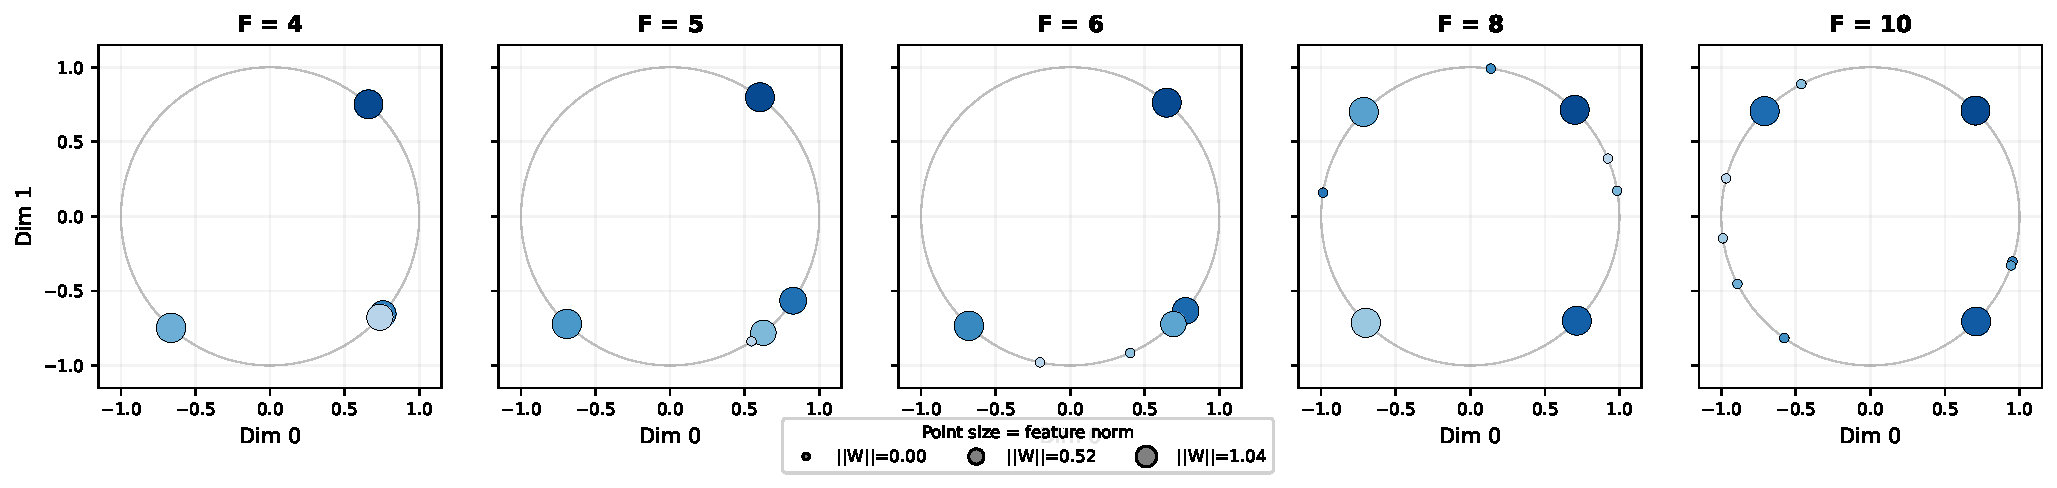
\includegraphics[width=\textwidth]{report_figures/fig1_polytopes.pdf}
\caption{Feature embeddings on the unit circle for $d{=}2$, $\alpha{=}1.0$,
seed 42. Point size is proportional to $\|W_i\|$; color encodes feature index.
The model discovers antipodal pairs (digons) at $F{=}4$, and progressively denser
angular packings as $F$ increases.}
\label{fig:polytopes}
\end{figure*}

The model reliably discovers structured arrangements (\Cref{fig:polytopes}).
At $F{=}4$, all three seeds produce two antipodal pairs (digons) --- the
optimal packing of 4 directions in 2D. At $F{=}5$, the model finds a pentagon
or a digon-plus-triangle arrangement depending on the seed. At $F{=}6$, three
digons or two triangles appear. All three seeds produced structured arrangements at these small $F$ values.

A key observation: point sizes in \Cref{fig:polytopes} reveal that the model
does not represent all features equally. At $F{=}8$ and $F{=}10$, rare features
(small circles, yellow) are pushed to near-zero norm while frequent features
(large circles, purple) maintain large norms.

SAE recovery in the $d{=}2$ regime is near-perfect: weighted MMCS exceeds
0.998 for all $F$ values (Table~\ref{tab:polytope}), --- clean geometry makes the SAE's job easy.

\begin{table}[h]
\caption{$d{=}2$ polytope sweep (mean $\pm$ std, 3 seeds).}
\label{tab:polytope}
\centering
\small
\begin{tabular}{rcccc}
\toprule
$F$ & EV & wMMCS & Dead\% & FRR \\
\midrule
4  & $.987 \pm .002$ & $\mathbf{.998} \pm .003$ & 38\% & 1.00 \\
5  & $.987 \pm .003$ & $\mathbf{1.00} \pm .001$ & 22\% & 1.00 \\
6  & $.986 \pm .004$ & $\mathbf{1.00} \pm .000$ & 32\% & 1.00 \\
8  & $.988 \pm .001$ & $\mathbf{1.00} \pm .000$ & 22\% & 0.96 \\
10 & $.989 \pm .001$ & $\mathbf{.999} \pm .001$ & 23\% & 1.00 \\
\bottomrule
\end{tabular}
\end{table}

\subsection{Power-Law Exponent Controls Representation Allocation}
\label{sec:alpha}

\textbf{Hypothesis:} Higher $\alpha$ steepens the frequency distribution,
concentrating $\|W_i\|$ on the most frequent features and leaving rare features
unrepresented.

\begin{figure}[h]
\centering
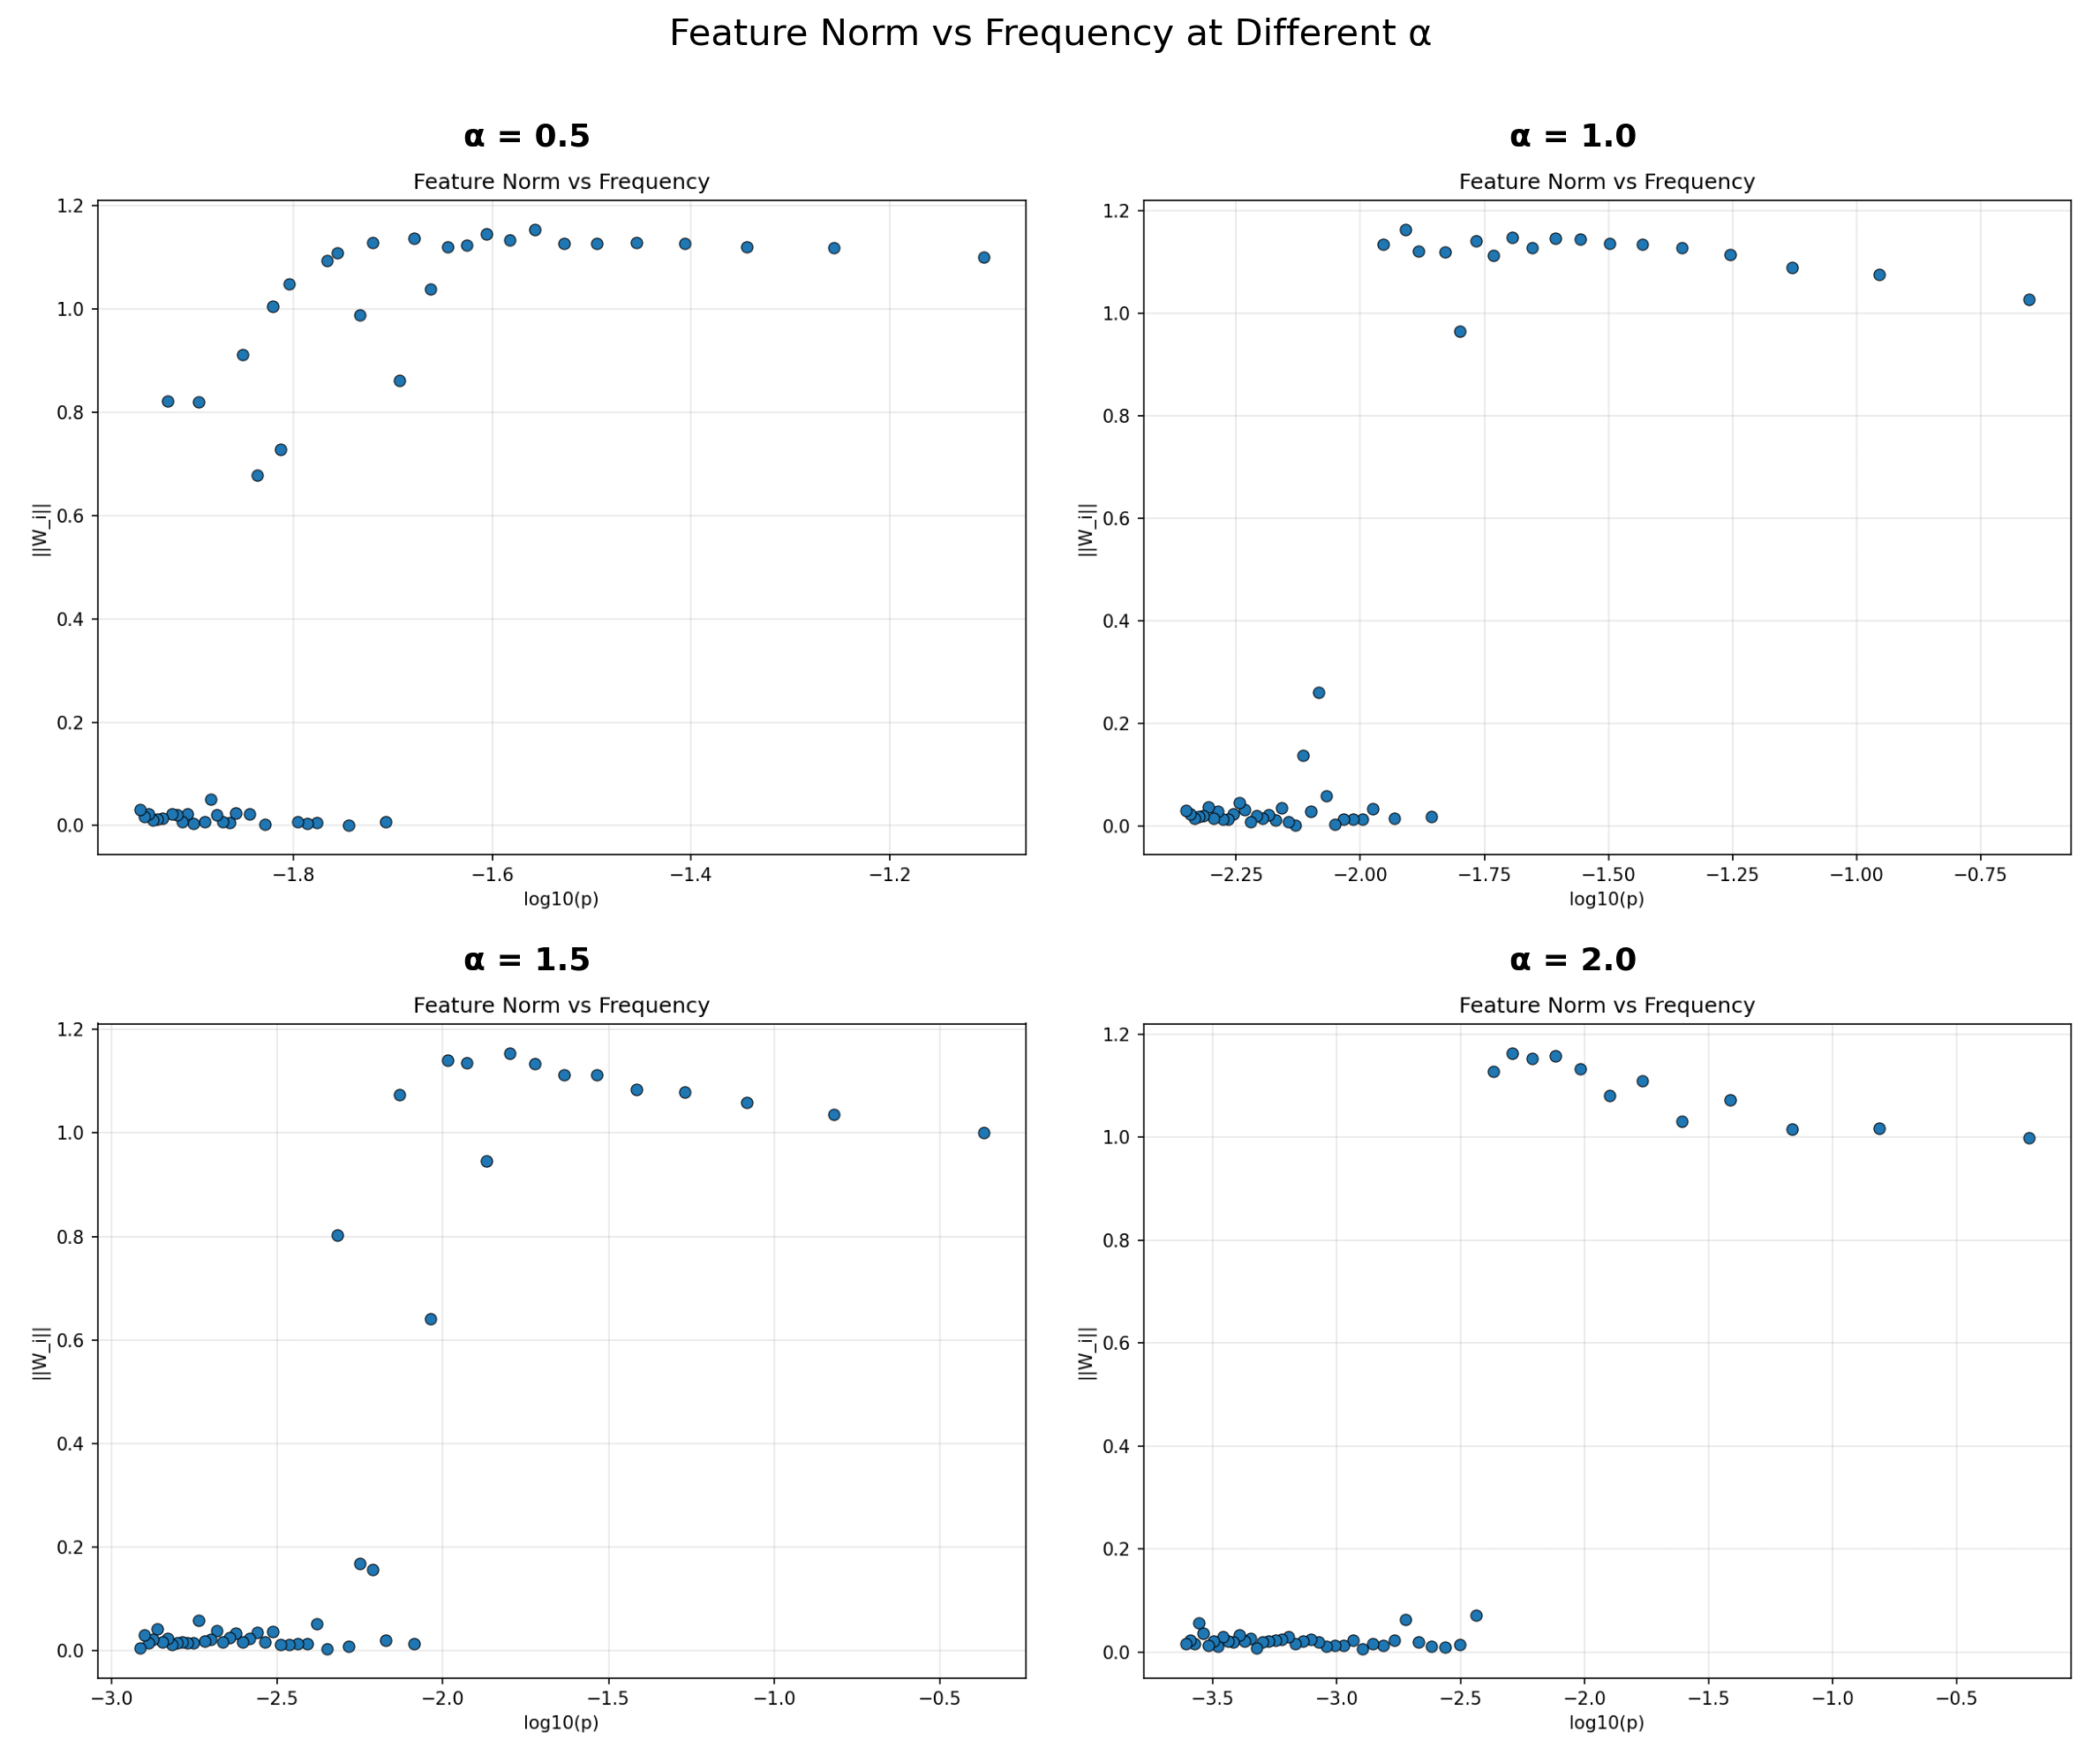
\includegraphics[width=\columnwidth]{report_figures/fig2_wnorms_alpha.png}
\caption{$\|W_i\|$ vs $\log_{10}(p_i)$ for $\alpha \in \{0.5, 1.0, 1.5, 2.0\}$,
$F{=}50$, $d{=}5$.}
\label{fig:wnorms}
\end{figure}

\Cref{fig:wnorms} shows this directly. At $\alpha{=}0.5$ (flat
distribution), feature norms spread across a wide range with no clear threshold.
At $\alpha{=}2.0$, there is a sharp step: the top $\sim$10 features have
$\|W_i\| \approx 0.7\text{--}0.9$, and the rest collapse to $\|W_i\| < 0.1$.

Higher $\alpha$ also improves weighted MMCS: $0.911 \pm 0.009$ at $\alpha{=}0.5$
versus $0.969 \pm 0.007$ at $\alpha{=}2.0$ (Table~\ref{tab:alpha}). Higher $\alpha$ improves wMMCS despite sacrificing more features: the survivors have high $\|W_i\|$ and well-separated directions, which the SAE finds easily.

Note that $\mathbb{E}[\|f\|_0] = \sum_i p_i = 1.0$ for all $\alpha$ by
construction (the normalization constant $C$ ensures this). The discriminating
quantity is the entropy $H(p) = -\sum p_i \log p_i$, which drops from 3.77 at
$\alpha{=}0.5$ to 1.52 at $\alpha{=}2.0$ (Table~\ref{tab:alpha}). Lower
entropy means more concentrated activations: at $\alpha{=}2.0$, the top 5
features account for 90\% of the probability mass. Recovery improves because the distribution is more peaked, not because it is sparser.

\begin{table}[h]
\caption{$\alpha$ sweep, $F{=}50$, $d{=}5$ (mean $\pm$ std, 3 seeds).
$H(p)$: entropy of feature probability distribution.}
\label{tab:alpha}
\centering
\small
\begin{tabular}{rcccc}
\toprule
$\alpha$ & $H(p)$ & EV & wMMCS & FRR \\
\midrule
0.5 & 3.77 & $.987$ & $.911 \pm .009$ & 0.53 \\
1.0 & 3.20 & $.989$ & $.937 \pm .007$ & 0.68 \\
1.5 & 2.30 & $.990$ & $.955 \pm .006$ & 0.73 \\
2.0 & 1.52 & $.991$ & $\mathbf{.969} \pm .007$ & 0.80 \\
\bottomrule
\end{tabular}
\end{table}

\subsection{Cosine Similarity Characterizes Superposition Regime}
\label{sec:cossim}

As $F/d$ increases, the pairwise cosine similarity distribution of $W$ columns transitions from structured to random-like (\Cref{fig:coshist}).

\begin{figure*}[t]
\centering
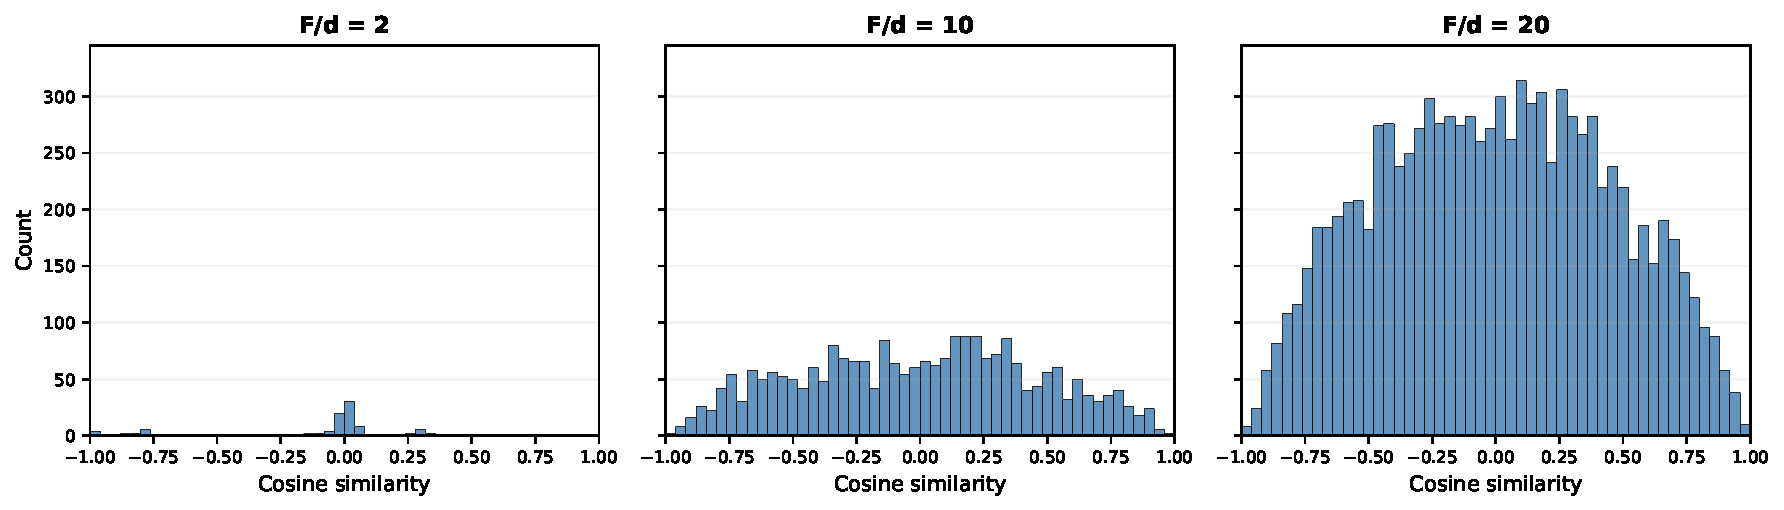
\includegraphics[width=\textwidth]{report_figures/fig3_coshist.pdf}
\caption{Off-diagonal cosine similarity distributions at $F/d = 2$, $10$, and $20$
($d{=}5$, $\alpha{=}1.0$). Shared y-axis scale across panels.}
\label{fig:coshist}
\end{figure*}

\Cref{fig:coshist} shows the transition. At $F{=}10$ ($F/d{=}2$), the
distribution is wide with visible structure --- some feature pairs are
near-orthogonal, others near-parallel. At $F{=}50$ ($F/d{=}10$), the
distribution narrows and centers near zero. At $F{=}100$ ($F/d{=}20$),
it becomes approximately Gaussian with standard deviation $\sim$0.25.

The feature dimensionality metric $D_i = \|W_i\|^2 / \sum_j (\hat{W}_j \cdot W_i)^2$
tells the same story (\Cref{fig:featdim}). At $F{=}50$, $d{=}5$,
most features have $D_i$ below 0.1, far below the dedicated ($D{=}1$), digon
($D{=}0.5$), and triangle ($D{=}2/3$) reference lines. The model operates
firmly in deep superposition.

\begin{figure}[h]
\centering
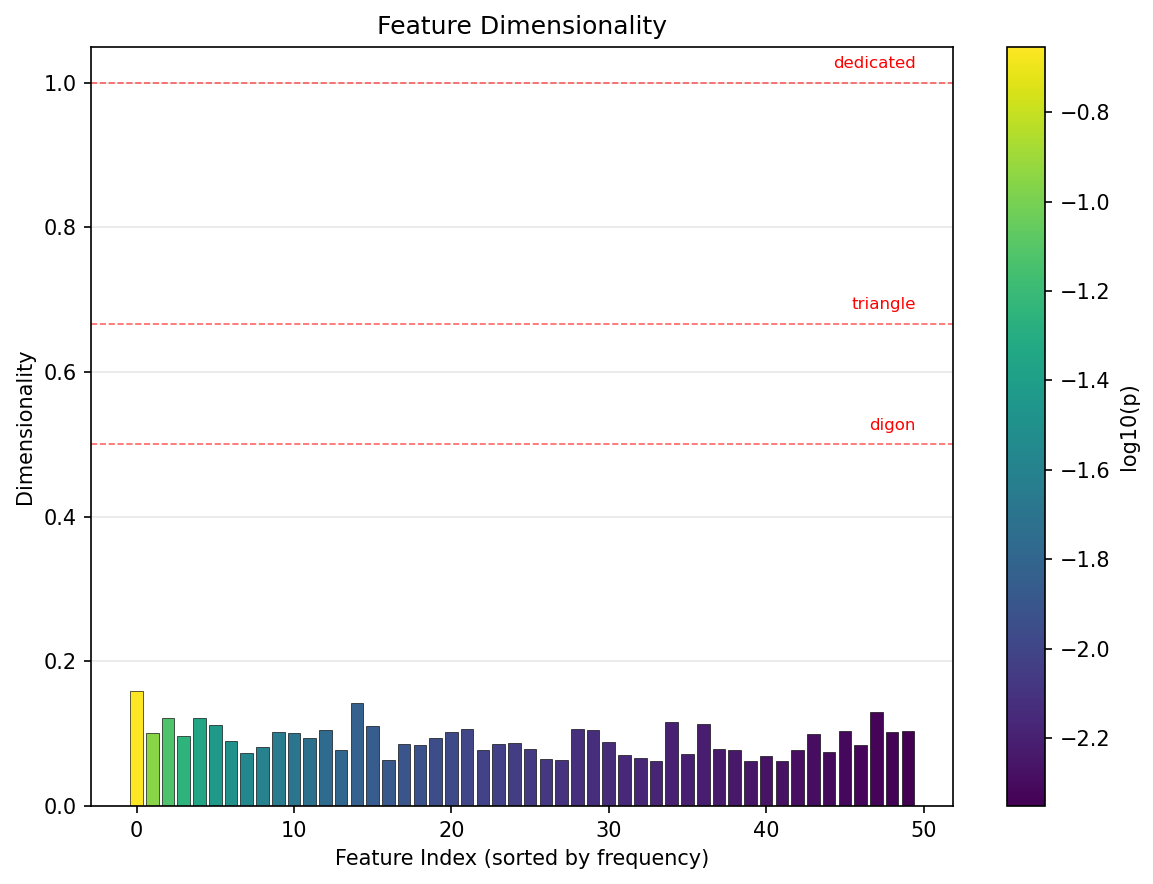
\includegraphics[width=\columnwidth]{report_figures/fig3_feat_dim.png}
\caption{Per-feature dimensionality for $F{=}50$, $d{=}5$, $\alpha{=}1.0$.
Horizontal lines mark dedicated ($D{=}1$), digon ($D{=}0.5$), and triangle
($D{=}2/3$) regimes.}
\label{fig:featdim}
\end{figure}

\subsection{Training Dynamics}
\label{sec:dynamics}

The assignment asks how training steps affect geometry. I trained the
toy model ($F{=}50$, $d{=}5$, $\alpha{=}1.0$) for 10k steps and examined $W$
at checkpoints 500, 1k, 2k, 5k, and 10k (Figure~\ref{fig:dynamics}).

\begin{figure}[h]
\centering
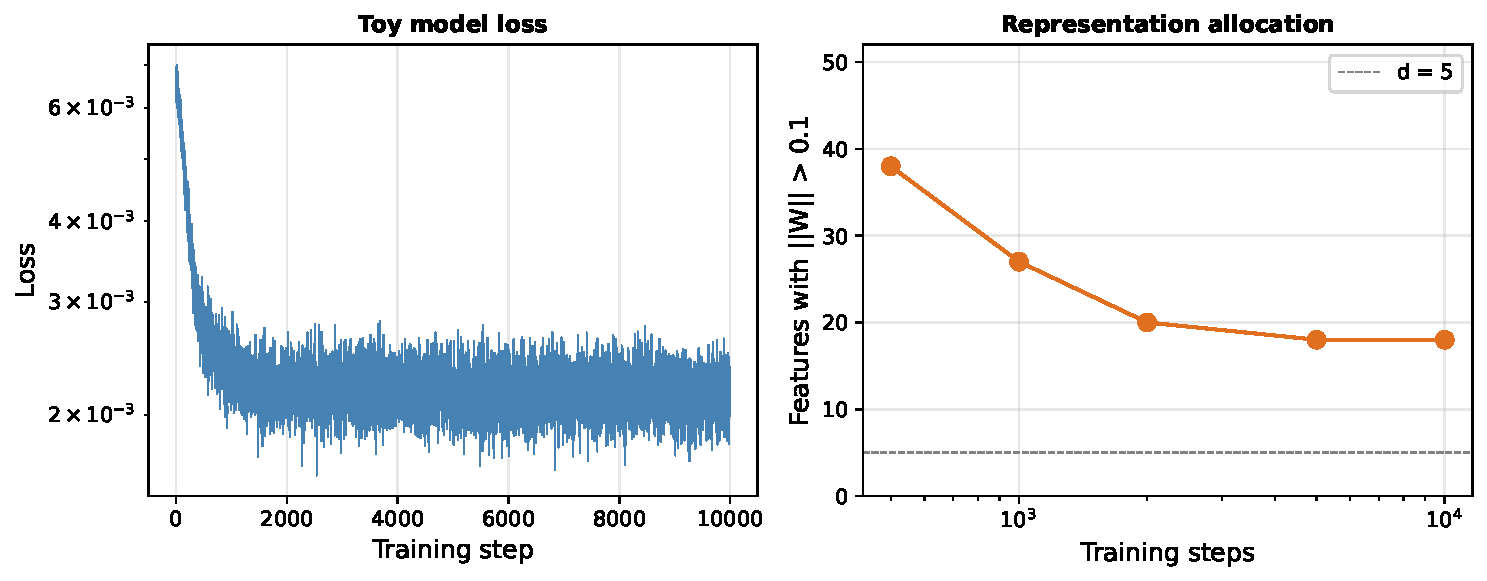
\includegraphics[width=\columnwidth]{report_figures/fig_training_dynamics.pdf}
\caption{Left: toy model loss over 10k steps. Right: number of features
with $\|W_i\| > 0.1$ at each checkpoint.}
\label{fig:dynamics}
\end{figure}

The loss converges by approximately 2k steps (Figure~\ref{fig:dynamics}, left),
dropping from $10^{-2}$ to ${\sim}2.2 \times 10^{-3}$ and changing negligibly
thereafter. The geometric structure, however, continues evolving: the model
starts by representing 38 features at step 500, then progressively discards
rare features, stabilizing at 18 represented features by step 5k. So loss converges first (${\sim}$2k steps), but the model keeps pruning features for another ${\sim}$3k steps after that. The final count of 18 represented features, well above $d{=}5$,
confirms that the model operates in the superposition regime even after
convergence.


\subsection{Hidden State Structure}
\label{sec:hidden}

The hidden states $h = W^T f$ inherit structure from both the feature
distribution and the learned embedding. Figure~\ref{fig:hidden} shows
the PCA spectrum of $h$ for different $\alpha$ values.

\begin{figure}[h]
\centering
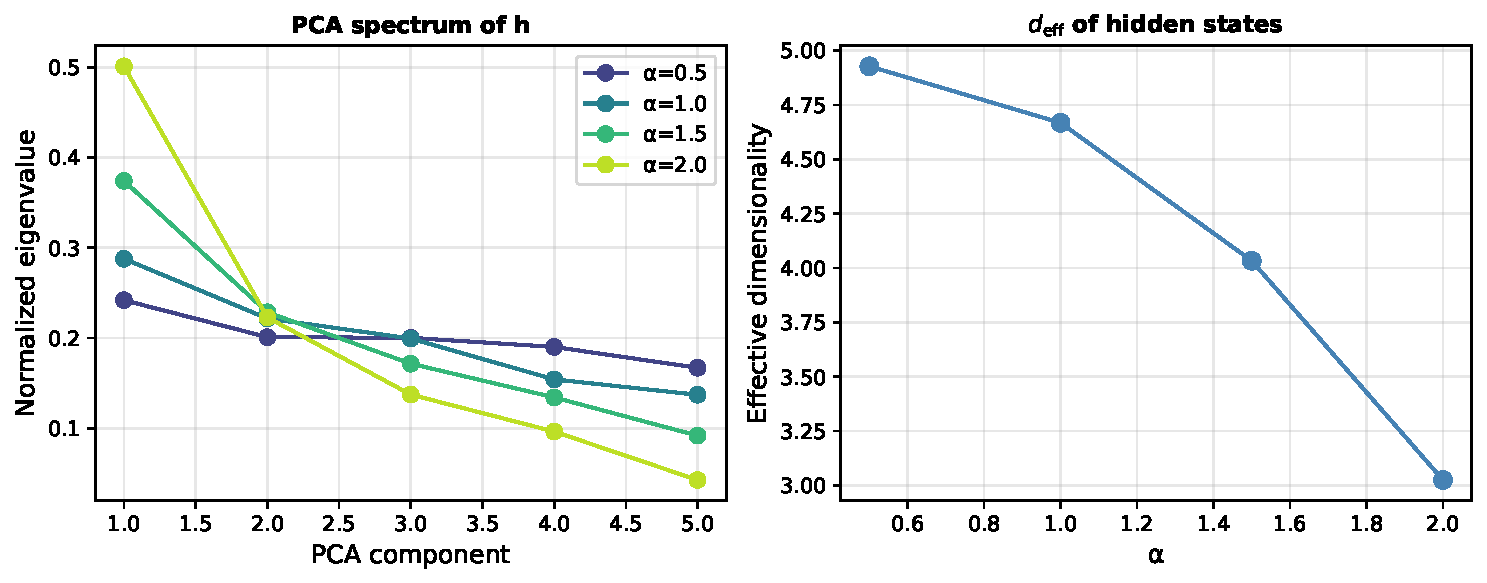
\includegraphics[width=\columnwidth]{report_figures/fig_hidden_states.pdf}
\caption{Left: PCA spectrum of $h$ for each $\alpha$ ($F{=}50$, $d{=}5$).
Right: effective dimensionality $d_\text{eff}$ (participation ratio) vs $\alpha$.}
\label{fig:hidden}
\end{figure}

At $\alpha{=}0.5$, variance is distributed nearly uniformly across all $d{=}5$
components ($d_\text{eff} = 4.93$). At $\alpha{=}2.0$, the first component
captures 50\% of variance and the last under 5\% ($d_\text{eff} = 3.02$).
This reflects the concentration: at high $\alpha$, only a few features
contribute meaningfully to $h$, so the hidden state occupies a
lower-dimensional subspace. Lower $d_\text{eff}$ means the SAE searches a smaller space, explaining the better recovery at high $\alpha$ (Table~\ref{tab:alpha}).


% ===================================================================
\section{Part 2: SAE Reconstruction Quality}
\label{sec:sae}

\subsection{The Sparsity--Fidelity Tradeoff}
\label{sec:l0}

\textbf{Hypothesis:} There exists a Pareto frontier between reconstruction
quality (EV) and sparsity ($L_0$), controlled by the $\ell_0$ coefficient.

\begin{figure}[h]
\centering
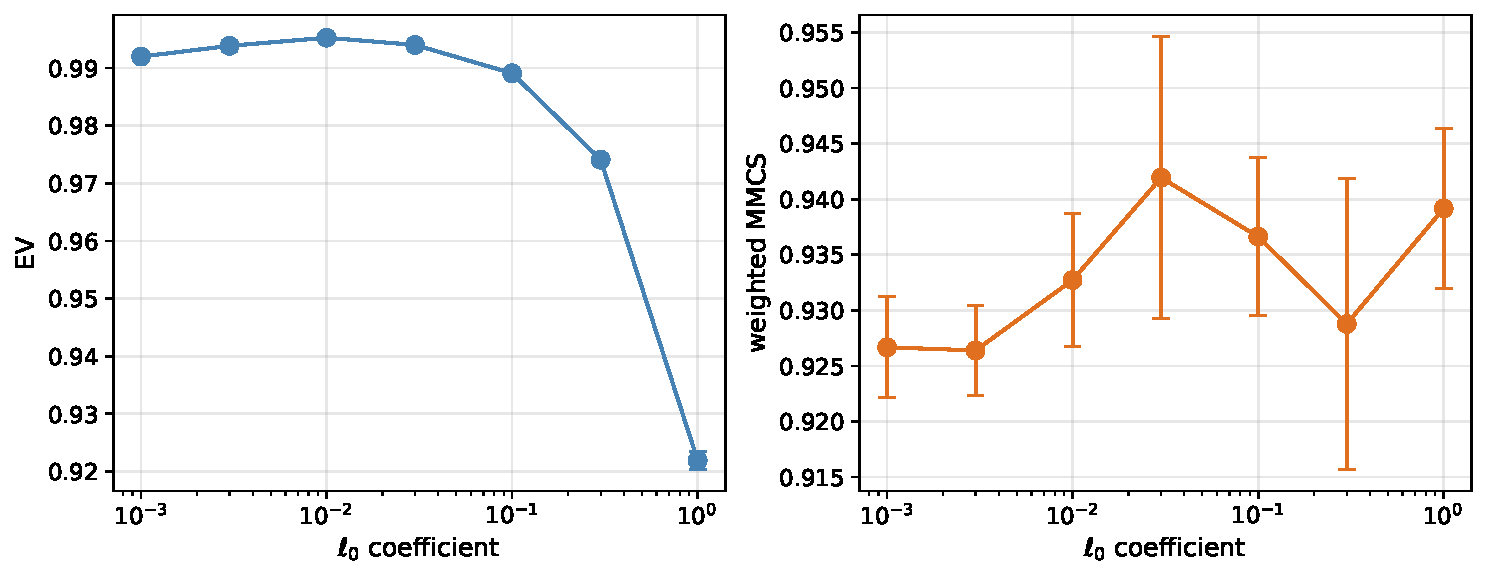
\includegraphics[width=\columnwidth]{report_figures/fig5_pareto.pdf}
\caption{Left: EV vs $\ell_0$. Right: weighted MMCS vs $\ell_0$. EV spans a 7.3~pp range while wMMCS varies by only 1.6~pp ($F{=}50$, $d{=}5$, $\alpha{=}1.0$).}
\label{fig:ev_l0}
\end{figure}

\Cref{fig:ev_l0} and Table~\ref{tab:pareto} confirm this. EV peaks at 0.995 near $\ell_0{=}0.01$ and degrades at higher sparsity,
reaching $0.922 \pm 0.002$ at $\ell_0{=}1.0$. The slight improvement from
$\ell_0{=}0.001$ to 0.01 suggests mild L1 regularization benefits reconstruction. The $L_0$ (mean active latents) drops correspondingly from
80.9 to 11.5.

\begin{table}[h]
\caption{Pareto frontier: $\ell_0$ sweep at $F{=}50$, $d{=}5$ (3 seeds).}
\label{tab:pareto}
\centering
\small
\begin{tabular}{rccccc}
\toprule
$\ell_0$ & EV & wMMCS & Dead\% & $L_0$ & FRR \\
\midrule
0.001 & .992 & .927 & 0.0 & 80.9 & 0.79 \\
0.003 & .994 & .926 & 0.0 & 50.8 & 0.75 \\
0.01  & .995 & .933 & 0.0 & 34.1 & 0.75 \\
0.03  & .994 & .942 & 0.3 & 30.0 & 0.74 \\
0.1   & .989 & .937 & 3.7 & 20.9 & 0.68 \\
0.3   & .974 & .929 & 8.3 & 15.9 & 0.61 \\
1.0   & .922 & .939 & 15.0 & 11.5 & 0.67 \\
\bottomrule
\end{tabular}
\end{table}

Weighted MMCS is stable across the full sweep: 0.926 to 0.942, a 1.6 percentage point range versus 7.3~pp for EV. The SAE learns the same decoder directions regardless of $\ell_0$.

\subsection{Dictionary Size Scaling}
\label{sec:fsae}

Larger dictionaries should help --- more capacity to decompose superposed representations.

\begin{figure}[h]
\centering
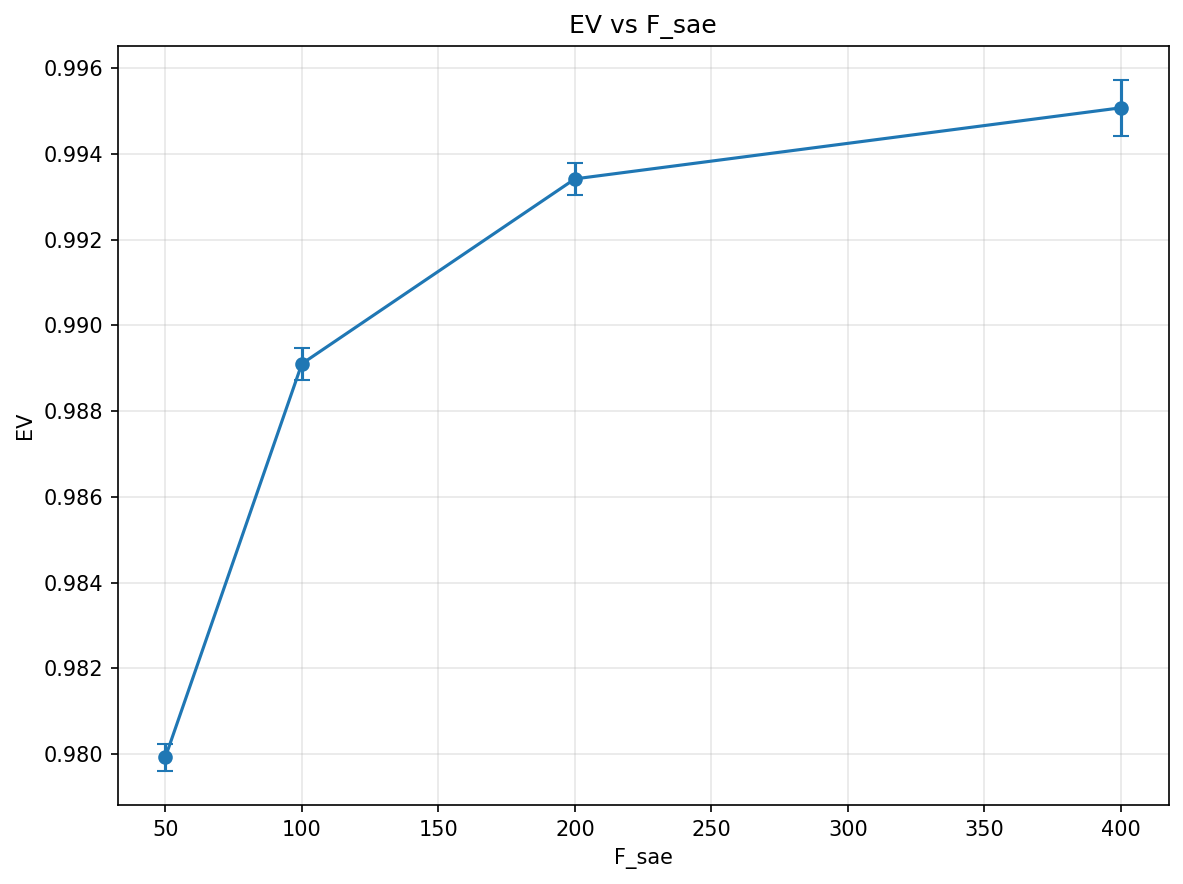
\includegraphics[width=\columnwidth]{report_figures/fig6_ev_vs_fsae.png}
\caption{EV vs $F_{\text{SAE}}$ ($F{=}50$, $d{=}5$, $\alpha{=}1.0$, $\ell_0{=}0.1$).}
\label{fig:ev_fsae}
\end{figure}

EV improves from $0.980 \pm 0.000$ at $F_{\text{SAE}}{=}50$ to
$0.995 \pm 0.001$ at $F_{\text{SAE}}{=}400$ (\Cref{fig:ev_fsae}).
More importantly, feature recovery rate (fraction with cosine $> 0.9$)
jumps from 0.44 at $F_{\text{SAE}}{=}50$ to 1.00 at $F_{\text{SAE}}{=}400$
(Table~\ref{tab:fsae}). MMCS improves correspondingly from 0.883 to 0.963.

\begin{table}[h]
\caption{Dictionary size sweep ($F{=}50$, $d{=}5$, 3 seeds).}
\label{tab:fsae}
\centering
\small
\begin{tabular}{rcccc}
\toprule
$F_{\text{SAE}}$ & EV & wMMCS & MMCS & FRR \\
\midrule
50  & $.980 \pm .000$ & $.903 \pm .006$ & $.883 \pm .007$ & 0.44 \\
100 & $.989 \pm .000$ & $.937 \pm .007$ & $.921 \pm .003$ & 0.68 \\
200 & $.993 \pm .000$ & $.954 \pm .002$ & $.945 \pm .002$ & 0.89 \\
400 & $.995 \pm .001$ & $\mathbf{.963} \pm .009$ & $.963 \pm .005$ & 1.00 \\
\bottomrule
\end{tabular}
\end{table}

At $F_{\text{SAE}}{=}400$ (8$\times$ overcomplete), every ground-truth
feature is recovered above the 0.9 cosine threshold. The price is a high
dead latent fraction (23.9\%) --- most of the 400 dictionary elements go unused.

\subsection{EV Is Not Discriminative}
\label{sec:ev_flat}

Across all experiments, EV exceeds 0.97 for every configuration except the
most aggressive sparsity penalty ($\ell_0{=}1.0$: EV $= 0.922$) and $d{=}10$
with high $\ell_0$ (Table~\ref{tab:d10}). So EV cannot distinguish an SAE that recovers everything from one that misses half the features.

The assignment asks whether properties of the learned $W$ matrix predict SAE
quality. Figure~\ref{fig:ev_W} plots EV against two summary statistics of $W$
across all 66 (config, seed) runs: mean absolute pairwise cosine similarity
(measuring feature interference) and effective rank (measuring how many
dimensions $W$ effectively uses).

\begin{figure}[h]
\centering
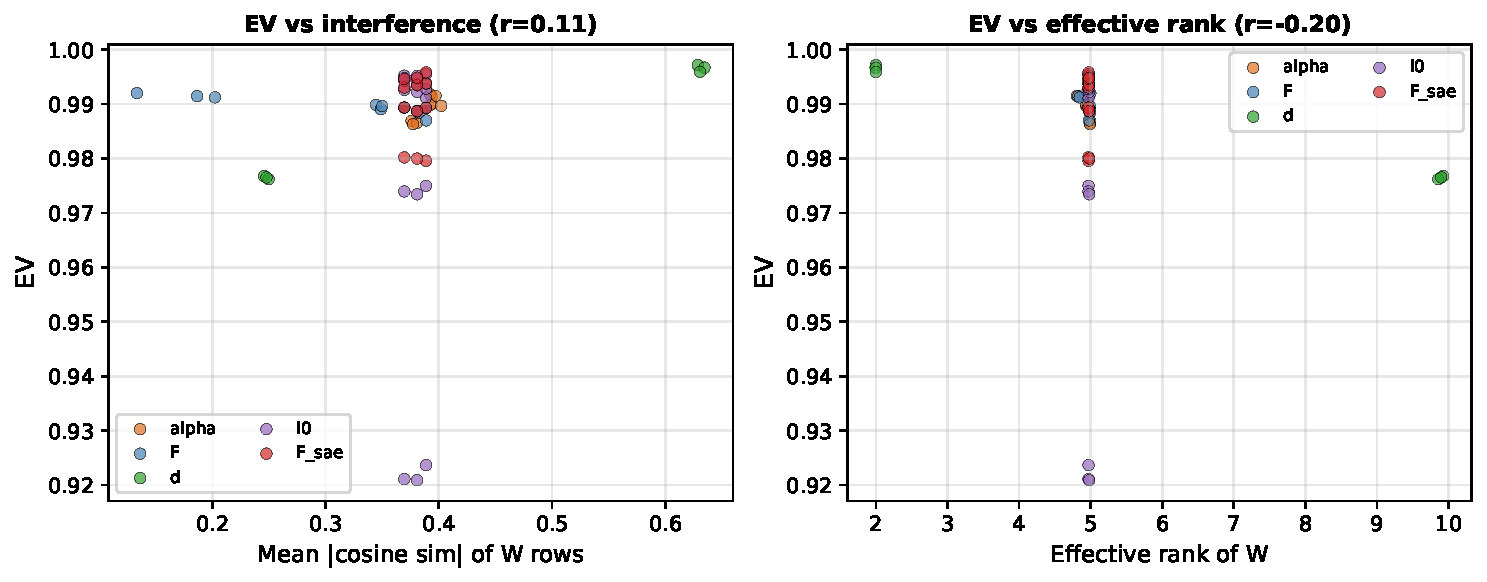
\includegraphics[width=\columnwidth]{report_figures/fig_ev_vs_W.pdf}
\caption{EV vs properties of $W$ across all sweep configurations.
Each point is one (config, seed) run, colored by sweep.}
\label{fig:ev_W}
\end{figure}

Neither metric correlates meaningfully with EV ($r = 0.11$ for interference,
$r = -0.20$ for effective rank). EV is primarily controlled by the SAE's own
hyperparameters ($\ell_0$, $F_\text{SAE}$) rather than by the toy model's
geometry. Again: EV does not tell you whether the SAE found the right features.

The $d{=}10$ regime is notable (Table~\ref{tab:d10}): at the default $\ell_0{=}0.1$,
weighted MMCS is only $0.803 \pm 0.012$ with a feature recovery rate of 18.7\%.
Increasing $\ell_0$ to 1.0 improves weighted MMCS to $0.881 \pm 0.025$ and
recovery to 52.7\%, at the cost of EV dropping from 0.977 to 0.832. At $d{=}10$ you need higher $\ell_0$ --- the default 0.1 is not enough.

\begin{table}[h]
\caption{$d{=}10$ operating point search ($F{=}50$, 3 seeds).}
\label{tab:d10}
\centering
\small
\begin{tabular}{rcccc}
\toprule
$\ell_0$ & EV & wMMCS & MMCS & FRR \\
\midrule
0.1 (default) & .977 & .803 & .802 & 0.19 \\
0.3 & .942 & .817 & .816 & 0.25 \\
0.5 & .908 & .830 & .829 & 0.33 \\
1.0 & .832 & $\mathbf{.881}$ & .877 & 0.53 \\
\bottomrule
\end{tabular}
\end{table}

\textbf{Synthesis.} EV above 0.97 is achievable across nearly all
configurations tested. The primary controls are the SAE's own parameters:
$\ell_0$ (which trades reconstruction for sparsity) and $F_\text{SAE}$
(which provides capacity). Model parameters ($\alpha$, $F/d$) have
minimal effect on EV but dramatically affect feature recovery
(Section~\ref{sec:recovery}). Properties of $W$ (interference, effective
rank) do not predict EV either. So EV does not reflect feature recovery quality.

% ===================================================================
\section{Part 3: Feature Recovery}
\label{sec:recovery}

\subsection{Rare Features Are Systematically Lost}
\label{sec:rare}

\textbf{Hypothesis:} The SAE preferentially recovers frequent features
(high $p_i$, high $\|W_i\|$) and systematically fails on rare features.

\begin{figure*}[t]
\centering
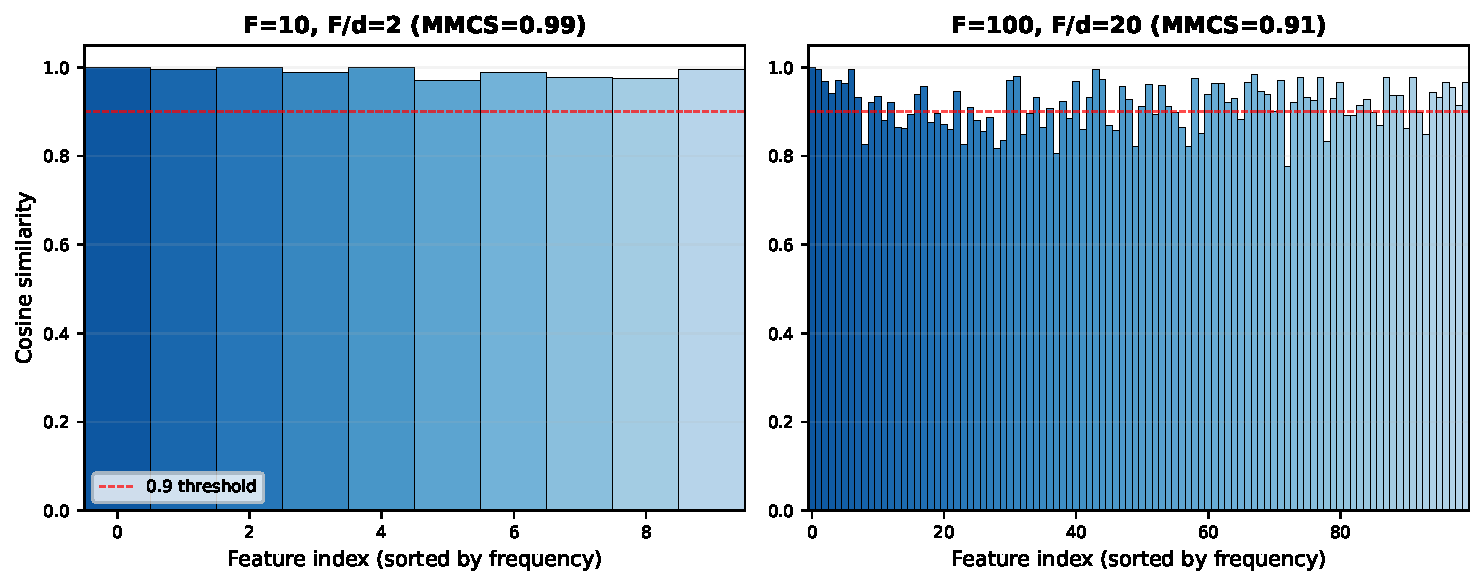
\includegraphics[width=\textwidth]{report_figures/fig7_mmcs_comparison.pdf}
\caption{Per-feature cosine similarity with matched SAE latent. Left: $F{=}10$ ($F/d{=}2$, near-perfect). Right: $F{=}100$ ($F/d{=}20$, selective recovery). Dashed line: 0.9 recovery threshold. Color encodes $\log_{10}(p_i)$.}
\label{fig:mmcs_compare}
\end{figure*}

\Cref{fig:mmcs_compare} makes this clear. At $F{=}10$ ($F/d{=}2$),
every feature achieves cosine similarity $> 0.95$ with its matched dictionary
element. At $F{=}100$ ($F/d{=}20$), the bar plot shows a clear bifurcation:
the first $\sim$15 features (highest frequency) are recovered well, while the
remaining $\sim$85 features have cosine similarities scattered between 0.6 and
0.95, with many below the 0.9 threshold.

\begin{figure}[h]
\centering
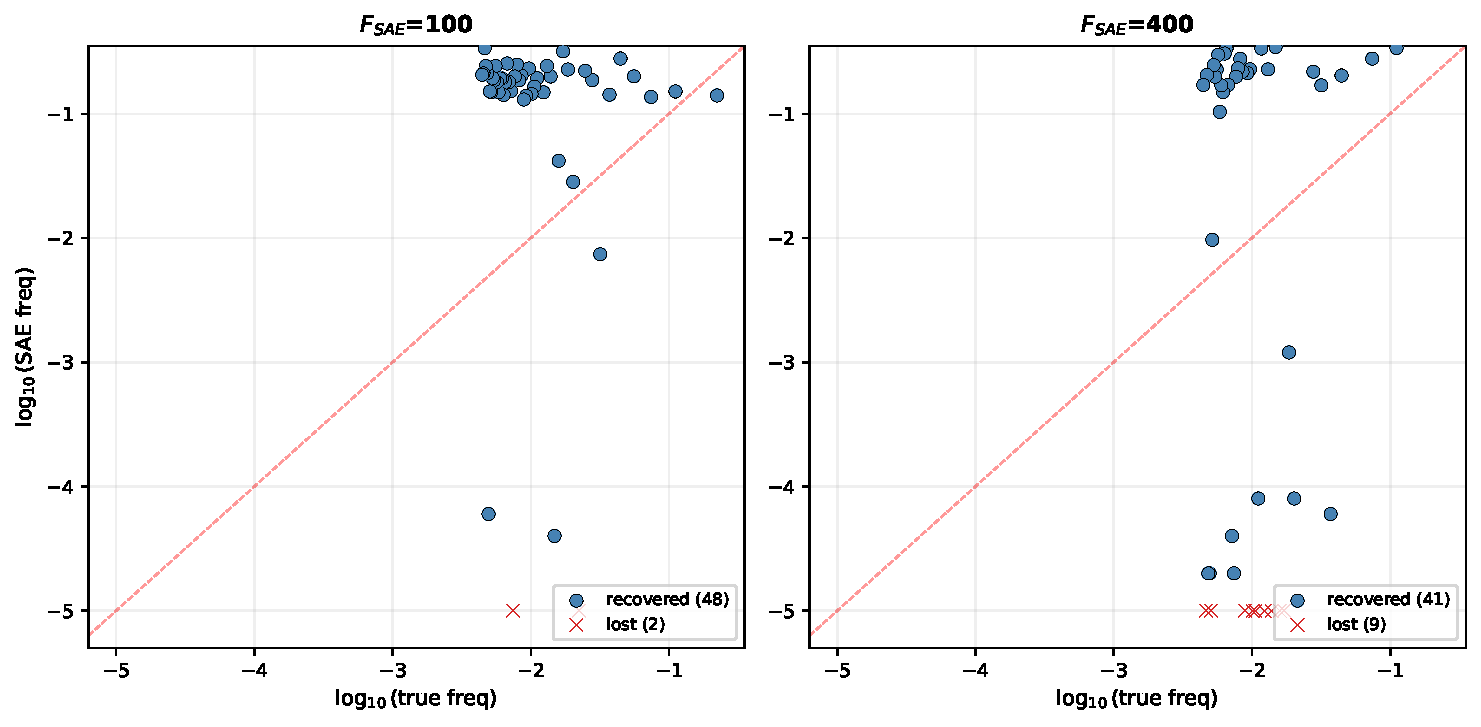
\includegraphics[width=\columnwidth]{report_figures/fig8_freq_recovery.pdf}
\caption{Frequency recovery scatter. Left: $F_{\text{SAE}}{=}100$ (default). Right: $F_{\text{SAE}}{=}400$ (8$\times$ overcomplete). At default dictionary size, rare features (high index, yellow) cluster at the bottom --- their matched SAE latents never fire. At 8$\times$ overcomplete, most features are recovered near the diagonal. Note: ``recovered'' here means the matched SAE latent has nonzero activation rate, not the cosine $> 0.9$ threshold used for FRR in the tables.}
\label{fig:freqrec}
\end{figure}

The frequency recovery scatter (\Cref{fig:freqrec}, left) shows the bifurcation: at default dictionary size ($F_{\text{SAE}}{=}100$), roughly 30 of 50 features cluster near the diagonal while the rest have SAE latents that never fire. At 8$\times$ overcomplete (\Cref{fig:freqrec}, right), nearly all features are recovered.

Feature recovery rate drops sharply with superposition depth:
1.00 at $F/d{=}2$, 0.68 at $F/d{=}10$, and 0.62 at $F/d{=}20$
(\Cref{fig:wmmcs}, left). At $F/d{=}20$, the SAE recovers only 62\% of features.

\subsection{$\ell_0$ Controls the Recovery Threshold}
\label{sec:l0_recovery}

While Section~\ref{sec:l0} showed that decoder directions are stable across
$\ell_0$, the feature recovery rate varies substantially: 0.79 at
$\ell_0{=}0.001$ down to 0.61 at $\ell_0{=}0.3$.

Low $\ell_0$ produces many active latents ($L_0 = 80.9$), meaning the SAE
distributes each hidden state across many dictionary elements. This improves
reconstruction but does not align dictionary elements with individual features.
Medium $\ell_0$ ($\sim$0.01--0.03) forces the SAE to use fewer, more
interpretable directions, improving per-feature alignment at minimal cost to EV.

\subsection{Superposition Depth Limits Recovery}
\label{sec:depth}

\begin{figure}[h]
\centering
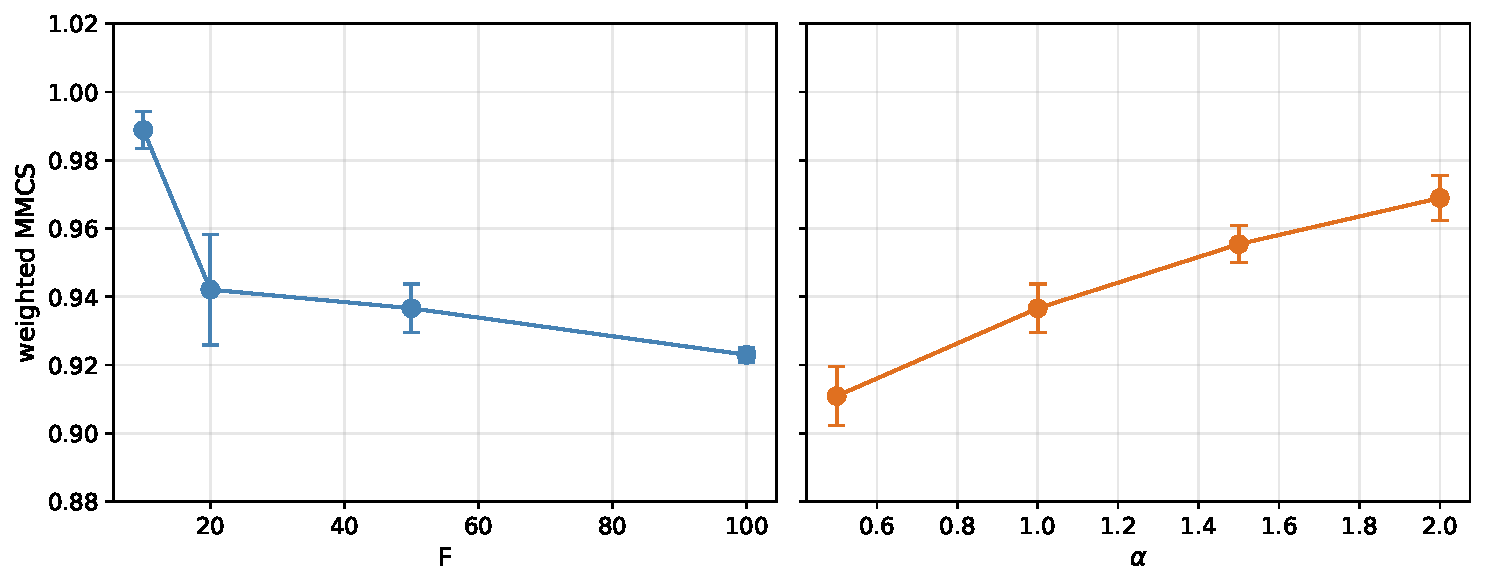
\includegraphics[width=\columnwidth]{report_figures/fig9_wmmcs_summary.pdf}
\caption{Weighted MMCS vs $F$ (left) and vs $\alpha$ (right). Mean $\pm$ std over 3 seeds. Y-axis zoomed to 0.88--1.02.}
\label{fig:wmmcs}
\end{figure}

The dominant constraint is $F/d$. Weighted MMCS degrades from
$0.989$ at $F/d{=}2$ to $0.923$ at $F/d{=}20$ (\Cref{fig:wmmcs}, left).
The degradation is smooth and consistent across 3 seeds.

The $d$ sweep reveals an asymmetry (Table~\ref{tab:dsweep}):
$d{=}2$ achieves near-perfect recovery (wMMCS $= 1.000$) while $d{=}10$
struggles (wMMCS $= 0.803$), even though both have $F/d{=}25$ and $F/d{=}5$
respectively. The $d{=}10$ regime has more room for superposition to spread
features across dimensions in non-axis-aligned ways, making SAE recovery harder.

\begin{table}[h]
\caption{Hidden dimension sweep, $F{=}50$, $\alpha{=}1.0$ (3 seeds).}
\label{tab:dsweep}
\centering
\small
\begin{tabular}{rccccc}
\toprule
$d$ & $F/d$ & EV & wMMCS & MMCS & FRR \\
\midrule
2  & 25 & $.997 \pm .001$ & $\mathbf{1.00} \pm .000$ & $.9997$ & 1.00 \\
5  & 10 & $.989 \pm .000$ & $.937 \pm .007$ & $.921$  & 0.68 \\
10 & 5  & $.977 \pm .000$ & $.803 \pm .012$ & $.802$  & 0.19 \\
\bottomrule
\end{tabular}
\end{table}

\subsection{EV and Feature Recovery Are Decoupled}
\label{sec:decoupled}

Consider two configurations:
at $d{=}2$, EV $= 0.997$ with weighted MMCS $= 1.000$ and FRR $= 1.00$.
At $d{=}10$, EV $= 0.977$ with weighted MMCS $= 0.803$ and FRR $= 0.19$.

The EV difference is 2 percentage points. The feature recovery difference is
81 percentage points. An SAE can explain 97.7\% of variance in the hidden states
while recovering fewer than 1 in 5 ground-truth features above the 0.9 cosine
threshold.

Similarly, in the $\ell_0$ sweep: EV spans 0.922--0.995 (7.3 pp range) while
weighted MMCS spans 0.926--0.942 (1.6 pp range) and FRR spans 0.61--0.79
(18 pp range). The metrics probe different aspects of SAE quality.

EV alone would have hidden the poor recovery in most of my experiments.

% ===================================================================
\section{Discussion}
\label{sec:discussion}

The 2D geometry is clean, and superposition scales smoothly with $F/d$ and $\alpha$. The SAE
recovers features reliably when superposition is mild ($F/d \leq 2$) but
degrades systematically at higher superposition ratios.

The main result is the EV--MMCS decoupling. EV can be near-perfect ($> 0.97$) while feature recovery is poor (wMMCS $< 0.85$). In my experiments, EV alone would have been misleading for almost every configuration.

The $d{=}10$ anomaly is not fully explained by these experiments. The fact that $d{=}2$
(higher $F/d{=}25$) achieves perfect recovery while $d{=}10$ ($F/d{=}5$)
struggles suggests that the difficulty of SAE recovery depends not just on the
superposition ratio but on the absolute dimensionality. In 2D, features must
lie on a circle --- a 1D manifold --- severely constraining the geometry and
making it easy for the SAE to find. In 10D, the space of possible feature
arrangements is vastly larger. This is a curse-of-dimensionality effect.

\paragraph{Limitations.}
This study uses uniform importance ($I_i = 1$), a vanilla SAE architecture
(no TopK, no Gated SAE), and relatively short training (10k--20k steps).
All experiments run on a single toy model class with power-law features.
All of this is on a toy model with independent Bernoulli features --- real transformer activations have correlated features and non-uniform magnitude distributions, so the specific numbers here should not be taken literally.

\paragraph{Possible extensions.}
If I had more time, I would try inverse-frequency importance weighting in the toy model loss --- the current uniform $I_i = 1$ systematically disadvantages rare features, and fixing that might be the cheapest way to improve tail recovery.

% ===================================================================

\end{document}
